\subsection{Généralités}
\label{subsec:generalites}

Tout lanceur à deux étages doit se reporter au cahier des charges \gls{Fusex} ainsi qu'à des règles supplémentaires. Une partie
du travail de la partie mécanique est de confirmer l'ensemble des étapes de conception et de fabrication. Les règles issues du
\acrshort{CDC} rappellent les conditions de validation afin de nous assurer de la conformité de nos systèmes tels que la tenue
mécanique, le double empennage, la flèche, le bon dimensionnement des parachutes... \\

Ce premier tableau ci-dessous récapitule les règles de structure globale afin de définir l'ensemble de nos matériaux pour les
composants soumis à de fortes contraintes.

\begin{table}[h!]
\centering
\begin{tabular}{|p{1.2cm}|p{4cm}|p{10cm}|}
\hline
Règles & Type & Détails du cahier des charges \\ \hline

MEC1  & Flèche & Les flèches statiques de l’étage 2 et de l’ensemble doivent être inférieures ou égales à 1\% (10 mm/m) \\ \hline
MEC2  & Tenue en compression & Chaque élément de l’étage 2 et de l’ensemble doit pouvoir supporter une compression équivalente à F = 2 x Accélération Max x Msup (en N) \\ \hline
MEC3  & Résistance longitudinale des ailerons & Les ailerons doivent pouvoir supporter une force longitudinale de : F = (2 x Masse d’un aileron x Accélération Max) + (0,02 x Surface d’un aileron x Vmax² x Coefficient de traînée) \\ \hline
MEC4  & Résistance transversale des ailerons & Une force F = 0,1 x Surface d’un aileron x Vmax$^2$ (en NEWTON) doit entraîner une flèche transversale des ailerons inférieure à 10° \\ \hline
MEC5  & Alignement des ailerons & Alignements des ailerons par rapport à l’axe longitudinal de la fusée < 1° \\ \hline
MEC6  & Angle entre deux ailerons & Angle entre deux ailerons consécutifs : 90° ± 10° (fusex à 4 ailerons) ou 120° ± 10° (fusex à 3 ailerons) \\ \hline
MEC7  & Tenue en traction & L’étage 2 et l’ensemble doivent rester intègres quand ils sont soulevés verticalement par l'ogive les ailerons vers le bas et par les ailerons l'ogive vers le bas \\ \hline
MEC8  & Double jeu d'ailerons & Dans le cas d’une fusée à deux jeux d’ailerons, les deux jeux d’ailerons sont soumis aux règles MEC3, 4, 5 et 6 \\ \hline
MEC9  & Tenue mécanique globale & La tenue mécanique de tous les éléments de la fusée doit leur permettre de fonctionner correctement lorsqu’ils sont soumis aux perturbations du vol (accélérations, vibrations, ...) \\ \hline
[...] &[...] &[...] \\ \hline

\end{tabular}
\caption{Règles de structure mécanique globale issues du \acrshort{CDC} \gls{Fusex} \cite[p.~32-33]{CDC_BiEtage}}
\end{table}

Ces validations seront détaillées et confirmées lors des contrôles au C'Space. Il est donc impératif de bien définir une justification adéquate.
Selon la règle et le cas de figure, nous définirons une validation par calcul analytique ou par simulation.

\newpage


\subsubsection{Flèche}
\label{subsubsec:premier_etage}
La première règle la plus critique dans un projet de fusée biétage étant la flèche. Nous appelons flèche la distance pour laquelle le corps de la fusée entière s'incline par rapport à sa position théorique à l'horizontale.
Nous devons valider selon la longueur totale un pourcetage en statique et en dynamique.\\

Dans nos estimations, nous avons estimé une masse totale inférieure à 8,00 kg et nous déterminons une masse pour notre calcul dynamique et ainsi avoir un coefficent de sécurité qui sera bénéfique pour le jeu dans le système de sépération.\\

Afin de déterminer la force à appliquer à un mètre, on calcule le couple créé par le poids de la fusée au niveau de la base de
l’étage inférieur.

\begin{figure}[h!]
    \centering
    \begin{tikzpicture}
        \node at (0,0) {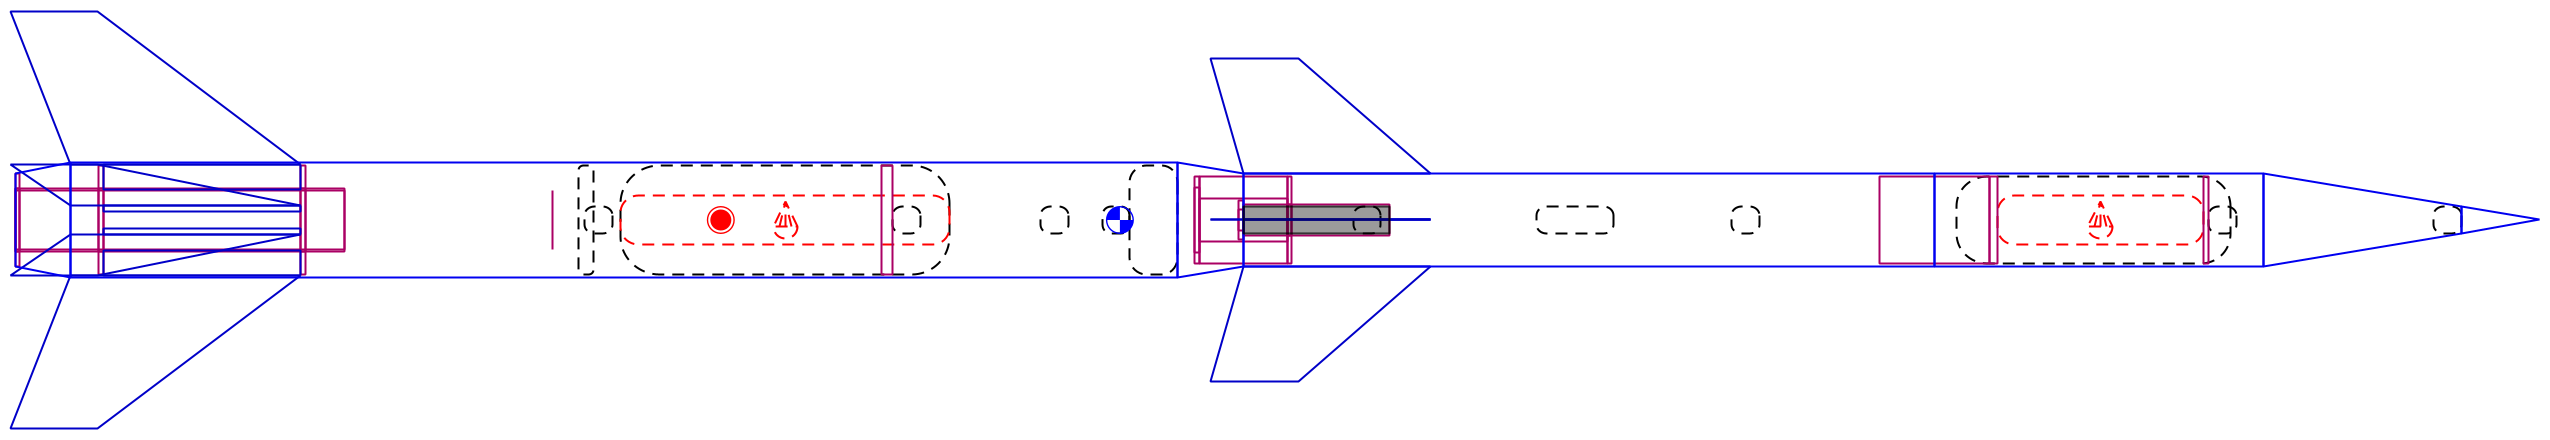
\includegraphics[width=\textwidth-0.75cm]{figures/SP_ork_narval-24.png}};

        \node (y_lbl)  at (-6.95, +0.500) {\textbf{y}};
        \node (x_lbl)  at (-6.70, -0.205) {\textbf{x}};
        \node (Cz_fbl) at (-6.60, +0.250) {\textbf{$C_z$}};
        \node (P_lbl)  at (-0.85, +1.000) {\textbf{P}};
        \node (F_lbl)  at (+6.00, +1.000) {\textbf{F}};

        \draw[red, <-, line width=1] (-7.200, +0.5) -- (-7.200, +0.0);
        \draw[red, <-, line width=1] (x_lbl.north)  -- (-7.200, +0.0);
        \draw[red, ->, line width=1] (+5.800, +1.0) -- (+5.800, +0.3);
        \draw[red, ->, line width=1] (-1.080, +1.0) -- (-1.080, +0.3);
        \draw[red, ->] (-6.7, 0) arc (0:90:.5cm);
        \draw [<->, > = stealth, black] (-7.2, -0.75) -- (-1.080, -0.75) node [midway, fill = white] {0,880m} ;
        \draw [<->, > = stealth, black] (-7.2, -1.25) -- (+5.800, -1.25) node [midway, fill = white] {1,960m} ;
    \end{tikzpicture}
    \caption{Schéma de calcul du couple exercé au niveau de la base du premier étage}
    \label{fig:placeholder}
\end{figure}

\begin{align*}
    P &= 9,81 \times 7,327 = 73,310\ N \\
    F &= 9,81 \times 0,8 = 7,848\ N\\
    \\
    C_Z &= 0,880 \times  (- P) + 1,960 \times (- F) \\
    &= 0,880 \times (- 73,310) + 1,960 \times (-7,848) \\
    &= -79,895\ N\cdotp m
\end{align*}
On a donc un couple de $-79,895\ N\cdotp m$, ce qui équivaut a :
$$\frac{|-79,895|}{9,81} = m_{test} \approx 8,144\ kg$$
$m_{test}$ étant la valeur de la masse à appliqués à un mètre du point d'encastrement pour reproduire le même couple.
Notre estimation de masse étant approximative, nous avons décidé d’arrondir la charge $m_{test}$ à $10\ kg$.\\

\underline{Validation physique (avant RCE3)}\\
À la suite de la conception, nous avons pu réaliser les tubes de la structure porteuse de la fusée. Nous avons procédé à un test
de flèche sur les tubes afin de nous assurer de la bonne tenue mécanique de ces derniers. Pour le tube du premier étage, nous
avons encastré le tube comme si tenu par le propulseur et réalisé les tests comme au \gls{C'Space}.\\

\begin{table}[h!]
    \centering
    \begin{tabular}{|c|c|c|}
        \hline
        Positionnement & Flèche statique & Flèche dynamique \\ \hline
        Patins à 0° & 0mm & 1mm \\ \hline
        Patins à 90° & 0mm & 1,5mm \\ \hline
        Patins à 180° & 0mm & 1mm \\ \hline
        Patins à 270° & 0mm & 2mm \\ \hline
        \end{tabular}
    \caption{Résultats des tests de flèche du tube du premier étage}
\end{table}

Les résultats montrent une flèche maximale de 0 mm en statique et 2 mm en dynamique pour une longueur de 1 m de tube. Cela 
correspond à une flèche relative de 0 \% en statique et 0,2 \% en dynamique, ce qui est largement en dessous de la limite de
1 \% imposée par le \gls{CDC} \cite[p.~32]{CDC_BiEtage}

\newpage


\subsubsection{Tenue en compression/traction}
\underline{Tenue en compression}\\
La tenue en compression permet de caractériser la force à appliquer sur la structure afin de simuler l'effort aérodynamique (pression de l'air ambiant lors de l'accélération maximale).
Afin de caractériser et de valider la tenue en compression, nous définissons la formule suivante :
\begin{align*}
    F_{comp} &= 2 \times Acc_{max} \times m_{tot} \\
    F_{comp} &= 2 \times 83 \times 10 = 1600\ N
\end{align*}
Ceci nous indique donc que l'ensemble de la structure et des composants environnants doivent supporter une force de 1600 N soit l'équivalent de \textbf{163,15 kg}. Lors des tests en contrôle, il faudra l'appliquer sur l'ensemble de la structure (de préférable depuis la coiffe du second étage).\\

\underline{Tenue en traction}\\
La tenue en traction nécessite que l'ensemble des équipements tient lorsque la fusée se trouve maintenue par la coiffe (ailerons vers le bas) et en sens inverse où la fusée est maintenue coiffe vers le bas par les ailerons du premier étage.


\subsubsection{Résistance des ailerons}
\underline{Résistance longitudinale}\\
La résistance longitudinale mesurée sur le bord d'attaque de chaque aileron est testée pour valider sa fixation au corps du lanceur. La formule est la suivante :
\begin{align*}
    F &= (2 \times m_{aileron} \times Acc_{max}) + (0,02 \times S_{aileron} \times V_{max}^2 \times C_x)\\
    F &= (2 \times (2,271\times 10^{-1}) \times 83) + (0,02 \times (2,103\times 10^{-2}) \times 176^2 \times 0,6)\\
    F &= 45,52 N
\end{align*}
Ainsi, chaque aileron doit supporter \textbf{4,64 kg} sur son bord d'attaque pour le valider.\\

\underline{Résistance transversale}\\
La résistance transversale permet de confirmer deux choses : 
\begin{itemize}
	\item La résistance de la plaque caractérisant l'aileron et de sa fixation au tube
	\item La déformation de l'aileron, dont la flèche maximale autorisée est inférieure à 10°
\end{itemize}
La prise de mesure se fait de la manière suivante : les ailerons sont posés proche de chaque saumon et une force est appliquée sur le tube. À noter que cette force appliquée équivant à deux alierons. Soit donc la formule suivante :
\begin{align*}
    F &= 0,1 \times S_{aileron} \times V_{max}^2 \\
    F &= 0,1 \times (2,103 \times 10^{-2}) \times 176^2 \\
    F &= 65,14 N\\
    F_{tot} &= 2 \times F = 130,29 N
\end{align*}
Soit donc dans notre cas de mesure expérimentale, une force de 130,3 N (\textbf{$\approx$13,28 kg}) doit être appliquée sur le tube au plus proche de l'aileron à la normale des deux à mesurer.
\subsubsection{Alignement des ailerons}
Pour confirmer la règle MEC5 et MEC6 concernant l'alignement et l'inclinaison des ailerons, un guide a été conçu par jeu d'ailerons pour guider le collage des quatre ailerons en simultané afin d'éviter toute erreur lors de l'assemblage.\\
Ayant des ailerons en composite sur tube composite, nous avons fait le choix de coller à la résine époxy (compromis entre performance structurelle, aérodynamique et esthétique).

\newpage

\subsubsection{Définition du système d'ouverture/parachute}
\label{subsec:defpara}

Dans l'objectif de récupération de chaque étage, nous devons définir et valider nos deux systèmes de sauvegarde des lanceurs.
Ceux-ci sont définis par des trappes latérales actionnées par un servomoteur chacun.\\

Le tableau suivant récapitule les règles du \acrshort{CDC} nous concernant (règles concernant les ralentisseurs pilotés non
présentes) et devant faire l'objet d'une validation technique.

\begin{table}[h!]
    \centering
    \begin{tabular}{|p{1.2cm}|p{4cm}|p{10cm}|}
        \hline
        Règles & Type & Détails du \acrshort{CDC} \\ \hline
        REC1  & Système récupération & Chaque étage doit être équipé d’un système ralentisseur fiable permettant de réduire sa vitesse de descente. L’éjection du/des ralentisseurs doit être franche. \\ \hline
        REC2  & Système récupération & Les systèmes ralentisseurs des étages et de tout autre élément éjecté doivent permettre une arrivée au sol à une vitesse verticale comprise entre 5 m/s et 15 m/s, y compris dans le cas dégradé où les deux étages ne se sont pas séparés. \\ \hline
        REC3  & Cohérence du système & Les instants de déploiement des systèmes ralentisseurs doivent être compatibles avec l’expérience menée par le club. \\ \hline
        REC4  & Séparation transversale & Non utilisé. \\ \hline
        REC5  & Séparation latérale & La case contenant le système de récupération doit rester opérationnelle lorsqu’elle supporte en compression longitudinale une force : $F = 2 \times \text{Accélération}{\text{Max}} \times M_{\text{sup}}$ (numériquement, l’accélération en m/s$^2$ et la masse en kg donnent $F$ en newtons). \\ \hline
        REC6  & Assemblage trappe & En position fermée, la porte latérale ne doit pas dépasser du profil de l’étage. \\ \hline
        REC7  & Tenue en torsion & La porte ne doit pas s’ouvrir ou se bloquer lorsqu’on applique un couple de torsion de 1 N·m entre le haut et le bas de l’étage. \\ \hline
        REC8  & Vibrations & L’accélération et les vibrations de la fusée ne doivent pas modifier le fonctionnement des systèmes de récupération. \\ \hline
        REC9  & Tenue mécanique globale & Les systèmes de récupération utilisés doivent auparavant avoir été testés avec succès. \\ \hline
        REC10 & Solidité du parachute & Les ralentisseurs doivent être suffisamment solides pour résister au choc à l’ouverture. \\ \hline
        REC11 & Anneau anti-torche & Dans le cas de l’utilisation d’un parachute, celui-ci doit être équipé d’un anneau anti-torche (également appelé glisseur). \\ \hline
    \end{tabular}
    \caption{Règles de dimensionnement des systèmes de récupération issues du \acrshort{CDC} \gls{Fusex} \cite[p.~36-42]{CDC_BiEtage}}
\end{table}

La contrainte imposée par le \acrshort{CDC} est une vitesse de redescente comprise entre 5 et 15m/s pour les trois
configurations (étage 1, étage 2 et non séparé). De par les dimensions des deux étages, le premier sera en charge du retour
sous parachute de l'ensemble non séparé.
\begin{equation}
\begin{aligned}
    V_d &= \sqrt{\frac{2 M g}{\rho_0 C_x S}} \
    %V_d &= \sqrt{\frac{2 \times 7.2 \times 9.81}{1.3 \times 1 \times 0.65}}
\end{aligned}
\end{equation}

Avec la règle REC2, nous devons dimensionner les deux parachutes pour les cas suivant la forme des parachutes utilisés. De plus, l'ensemble du
parachute devra résister à l'ouverture, c'est-à-dire résister à une force critique appliquée :
\begin{equation}
\begin{aligned}
    F &= 2 \times Acc_{max} \times K_{safety} \times M_{sup} \\
\end{aligned}
\end{equation}

Nous garderons ces définitions pour le dimensionnement et la vérification de la tenue des deux parachutes.
\newpage
